\documentclass{article}
\usepackage[utf8]{inputenc}
\usepackage[english]{babel}
\usepackage{amsmath}
\usepackage{amssymb}
\usepackage{setspace}
\usepackage{natbib} 
\usepackage{graphicx}
\usepackage{subfig}
\usepackage{comment}
\usepackage[backgroundcolor=pink,linecolor=red]{todonotes}
\usepackage{fullpage}
\usepackage[hidelinks]{hyperref}
\usepackage{xcolor}


%\singlespacing
\onehalfspacing
%\doublespacing

\newcommand{\E}{\mathbb{E}}
\renewcommand{\P}{\mathbb{P}}

\newcommand{\plr}[1]{\todo[linecolor=blue,backgroundcolor=blue!25,bordercolor=blue]{#1}}
\newcommand{\jgg}[1]{\todo[linecolor=green,backgroundcolor=green!25,bordercolor=black]{#1}}
\newcommand{\bill}[1]{\todo[linecolor=green,backgroundcolor=yellow!25,bordercolor=black]{#1}}

\begin{document}

\title{A few stickleback suffice to transport adaptive alleles to new lakes}
\author{Jared Galloway, William A. Cresko, and Peter Ralph}
\maketitle


\section*{Abstract}

Threespine stickleback fish provide a striking example of local adaptation despite recurrent gene flow.
The species is distributed around the Northern hemisphere in both marine and freshwater habitats.
It is thought that these numerous, smaller freshwater populations
have been established ``de novo" from marine fish,
and that a shared freshwater phenotype
is often established using standing genetic variation.
Here we use genealogical simulations to determine the levels of gene flow
that best matches observed patterns of allele sharing among habitats in stickleback, 
and more generally to better understand how gene flow and local adaptation in large metapopulations
determine speed of adaptation and reuse of standing genetic variation.
We find that rapid, repeated adaptation using a shared set of alleles maintained at low frequency by migration-selection balance occurs over a realistic range of intermediate rates of gene flow.
Low gene flow leads to slow, independent adaptation of distinct habitats, whereas high gene flow leads to large migration load.
We quantify how $F_{ST}$ scans for adaptive alleles are more likely to succeed with higher rates of gene flow.
In addition, we find the origin of many freshwater adapted alleles in the introduced lakes to be propagated from the original generation of marine individuals that had inhabited the lake.
The results support existing theory of local adaptation, and provide a more concrete look at a particular, empirically motivated example.  
\plr{say transporter hypothesis?}
\plr{talk about linkage and haplotypes}

\section*{Introduction}

% Jared's general notes for formatting
%
% - ``citep'' for ``cite in parentheses''. (and, citations come before the punctuation)
% - in latex, use ` `words' ' to get the open- and closed-double quotes (not the double-quote character)
% - "citet" for "cite, as part of the text"

The canonical model for the genetics of adaptation, first formulated by Fisher in the early part of the 20th century, involves the sequential fixation of new mutations. 
While it has proven valid in numerous studies in the field as well as in the lab, this model is now rightfully understood as incomplete for many species in nature that have more complicated population structures. 
What role does genomic variation play in metapopulations with connection to an array of selective pressures?
How could migration-selection balance and ecological speciation actually benefit species as a whole?
A growing number of studies have identified instances of convergent or shared adaptive evolution in small demes that utilize standing genetic variation (SGV) found in the static population from which they split.
However, it is still widely unknown which variations of evolutionary processes such as gene flow, recombination, selection and mutation, promote the maintenance and re-use of such genetic polymorphisms.
In addition, we would like to know how complex geographic systems, with a variety of selective pressures, interact with these evolutionary forces to help or hinder the use of SGV in newly colonized subpopulations.
\plr{I like the spirit of the first paragraph, but want to totally rewrite it}

Recently, a large flood of data resulting from evolutionary systems of organisms have come from population genomic studies powered by advances in sequencing technologies. 
One such organism is the threespine stickleback. 
Many studies of species have exhibited a long standing evolutionary history of migration-selection balance between marine and freshwater populations across the globe.
The rigidity of the stickleback's ability to frequently prosper in newly created freshwater environments has made this fish a good model for understanding the genetic basis of adaptive evolution. 
The ancestral marine form of stickleback has given rise to millions of independently derived populations in recently de-glaciated regions of the Northern Hemisphere.
While geographic isolation prevents direct migration between a large majority of these patches of freshwater populations,
They appear to exhibit very similar phenotypes, as well as many shared, adaptive alleles often found to be identical by decent (IBD). 
Impressively, independent local adaptation of marine individuals to freshwater environments has been observed to take place in tens of generations, 
and the adaptive alleles are found in freshwater populations that have been geographically isolated since the end of the last ice age $\approx 13,000$ years ago (Cite Kristin).
For example, in 1964 the Great Alaskan Earthquake caused an uplift of Middleton island and in turn, introduced a group of freshwater ponds around the perimeter of the island. 
Quickly inhabited by the surrounding marine population of stickleback, 
\citet{lescak2015evolution} observed significant phenotypic changes in less than 50 years that appear to be parallel to freshwater stickleback that have been separated for over thousands of years. 
In these freshwater stickleback, the number of lateral plates are reduced and the opercle shapes shows
the same expansion of the dorsal region and reduction of the ventral region as observed in the large majority of freshwater demes.

But how can evolution occur at such a rapid pace? 
Waiting for new mutations to arise in each lake would take much longer, and the genotypes being identical by state is even more improbable. 
This would seem to suggest that freshwater alleles are maintained in the marine individuals allowing the accelerated selection on SGV found in marine individuals which colonize the lake. 
The first clear example of the global reuse of SGV was the gene \textit{eda} which has been shown to be an important regulator for the number of lateral plates. 
While the low lateral plate version of this gene arose millions of years ago, it is found in freshwater ponds which have formed much more recently. 
Contemporary population genomic studies employing genome-wide haplotype analyses has provided evidence that \textit{most} regions of the genome that distinguish marine-freshwater genetic differences share this pattern \citep{nelson2017ancient}. 
 
\citet{schluter2009genetics} formulated the ``transporter'' hypothesis to explain these observations,
a conceptual model in which alleles benefical in freshwater populations
are maintained at migration-selection balance in the larger oceanic population
and thus available for subsequent adaptation into new freshwater habitats.
The hypothesis seems fits available data,
but a number of quantitative questions remain.
Are the actual population sizes, migration rates, and fitness differentials
consistent with this hypothesis?
How many of these differentially selected alleles are there,
and how are they arranged within the genome?
Does adaptation to a new lake rely on presence of early-generation hybrids between freshwater and marine fish,
i.e., on long haplotypes recently inherited from freshwater-dwelling stickleback?
Or, is the process
more akin to the atomization and reconstruction effected by the Star Trek technology that motivated the hypothesis' name?
More generally, 
how do the dynamics and eventual genomic organization
depend on the level of gene flow and strength of local adaptation,
both across the entire stickleback metapopulation
and separately within each lake?

In this paper, we used forward simulations 
modeled on the threespine stickleback metapopulation
to ask how gene flow affects the genetic and genomic architecture of local adaptation.
We know in practice that stickleback populations in new habitats can adapt in only tens of generations \citep{middleton};
what level of between-habitat gene flow is required for such rapid adaptation?
Genome scans for between-habitat differentiation have detected a number of causal QTL;
what proportion of the loci actually underlying adaptation do we expect to be detected by such scans?
How does our power to detect causal loci depend on the amount of gene flow?

We find that only a few stickleback per generation, per lake, 
suffices to maintain sufficient genetic variation in the ocean
so that new freshwater populations can adapt from standing variation in only tens of generations.
We also find that continued gene flow of marine individuals into recently established lakes
is not important for adaptation,
and so it is only ``downstream'' gene flow that allows freshwater adaptations to be ``transported'' between lakes.
% We show that low levels of introgression also results in noise that often presents itself as $F_{st}$ peaks when scanning across the genome suggesting introgression plays a key role in inferring causal loci . 
This rapid, local adaptation can only occur over an intermediate range of levels of gene flow --
low gene flow prevents variation from being transported,
while high gene flow prevents local adaptation.


%%%%%%%%%%%%%%%%
\section*{Methods}

To explore these questions, we used SLiM \citep{haller2017slim,haller2018slim3} 
to implement forwards-time simulation of populations of individuals with explicitly represented genomes
in which selection acted upon a single continuous quantitative trait.
The details of the model were motivated by current understanding of threespine stickleback evolutionary history and demography,
and included divergent selection in the two habitats which had substantial spatial structure.
Certain aspects of the model remain simplistic due to computational constraints.
Possibly the most important caveat is that simulated population sizes 
are much smaller than the census size of the threespine stickleback populations observed in nature
(see the Discussion for more on this).

\paragraph{Habitat and geography}
Throughout the simulation there are two habitat types -- Marine and Freshwater-- defined by their selective pressures.
We start the simulations with two populations of size 5,000 diploid individuals in each of the habitats, for a total of 10,000 diploid individuals.
The arrangement of these habitats, depicted in Figure \ref{fig:Geo},
roughly models a set of freshwater habitats along a stretch of coastline. 
The marine habitat is a continuous, one-dimensional range of length 25 units,
while the freshwater habitat is divided into 25 discrete subpopulations (which we call ``lakes''),
each connected to the marine habitat at regularly spaced intervals
(positions $i - 1/2$ for $1 \le i \le 25$).

Divergent selection is mediated by a single quantitative trait
with different optima in marine and freshwater habitats.
This situation roughly models the cumulative effect of the various phenotypes such as armor morphology, 
body size, craniofacial variation and opercle shape on which divergent selection is thought to act on in the two environments. 
Concretely, the optimal trait values in the marine and freshwater habitats are $+10$ and $-10$ respectively,
and fitness of a fish with trait value $x_\text{ind}$ in a habitat with optimal value $x_\text{opt}$
is determined by a Gaussian kernel with standard deviation 15, i.e.,
\begin{align*}
    f(x_\text{ind}; x_\text{opt})
    &=
    \exp\left\{
        \frac{1}{2}
            \left(
            \frac{x_\text{ind}-x_\text{opt}}{15}
            \right)^2
        \right\} .
\end{align*}

In short, the difference between an individual's trait value and the optimum largely determines that individual's fitness. 
Note that the scale we measure trait on is arbitrary as only the scale of trait values relative to mutation effect size is relevant.
We chose the difference between optima and strength of stabilizing selection in each habitat
so that 
(a) around 10 (diploid, homozygous) mutations were sufficient to move from one optimum to the other,
and (b) well-adapted fish from one habitat would have low, but nonzero, fitness in the other habitat.

\begin{figure}
	\begin{center}
  		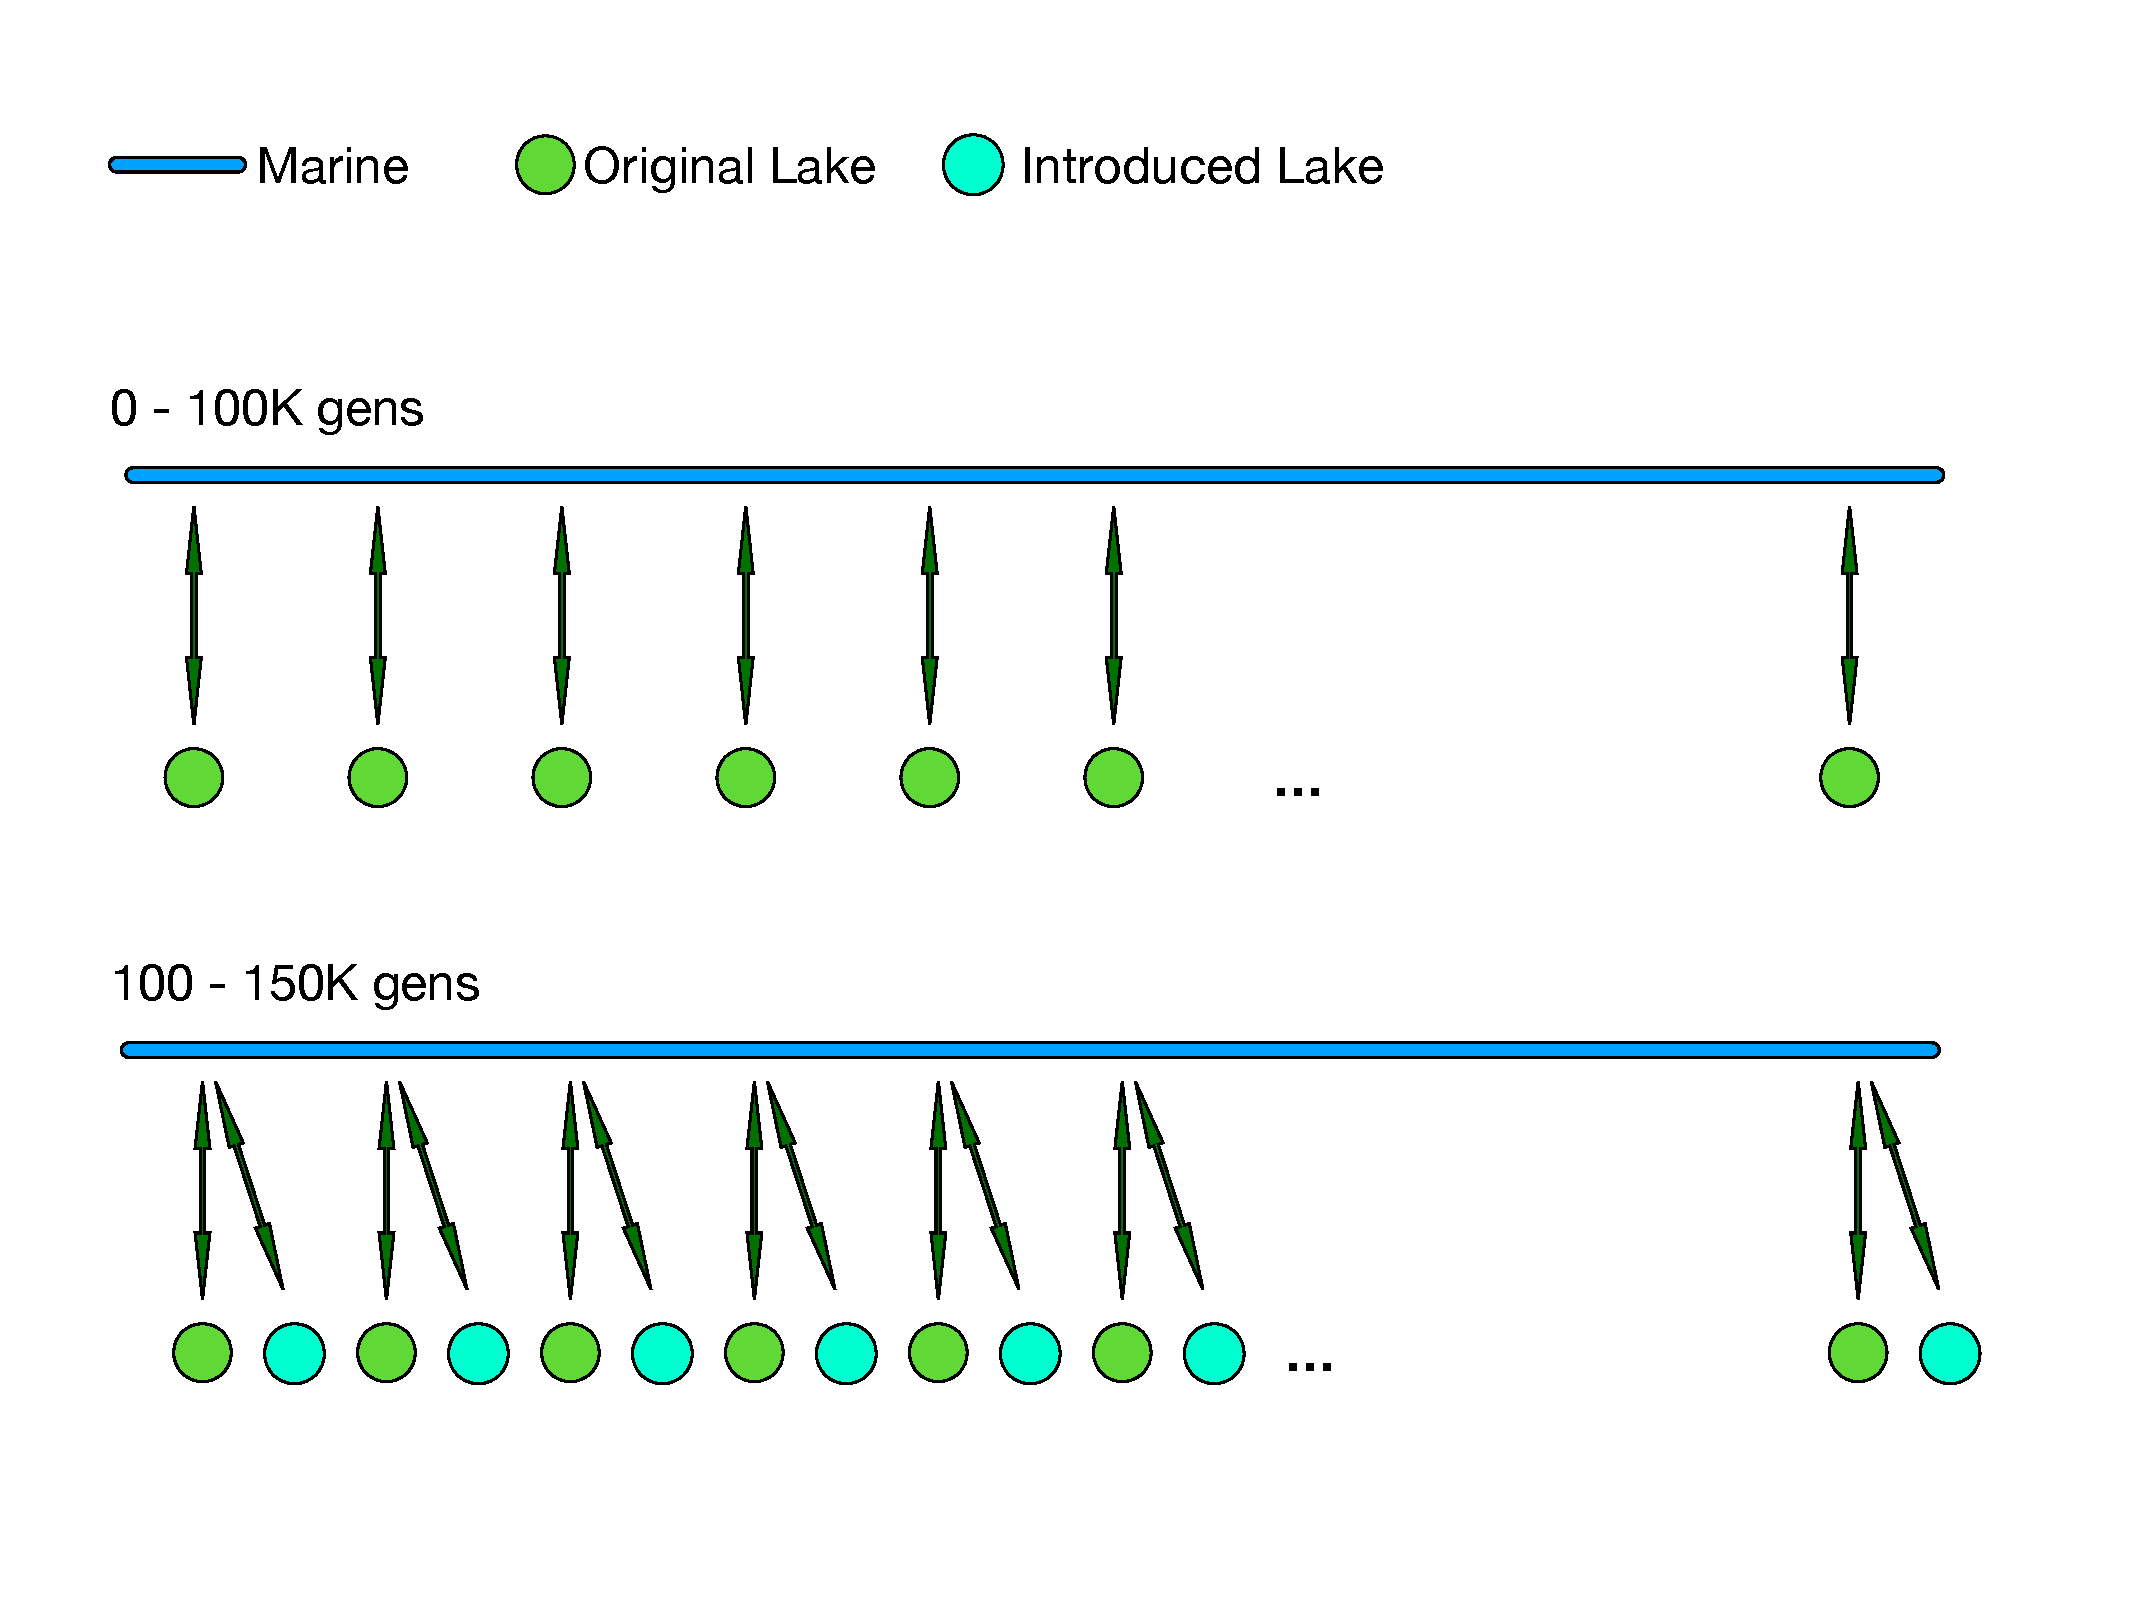
\includegraphics[width=0.6\linewidth]{GeographyFigure.pdf}
  		\caption{
            \textbf{Diagram of simulated populations:}
            a single, continuous, one-dimensional marine habitat (blue)
            is coupled to randomly mating ``lakes'' at discrete locations with dark green arrows representing migration patterns.
            After an initial period of 100K generations with 25 lakes,
            an additional 25 lakes are added (at the same set of locations) and populated with a copy of the \textit{marine} individuals
            to simulate the appearance of newly accessible freshwater habitats colonized by marine stickleback.
            The marine habitat, and each set of 25 lakes, each contain 5,000 individuals at all times.
			}
  		\label{fig:Geo}
	\end{center}
\end{figure}

\paragraph{Genetic architecture of the trait}
Each individual carries two linear chromosomes, each of size $10^8$ loci.
Mutations that can affect the trait under selection can occur at rate $10^{-7}$ per locus per generation
in ten ``effect regions'' of $10^5$ loci each,
spread evenly along the chromosome.
Each mutation in these regions is either additive, completely recessive, or completely dominant (with equal probability). 
Effect sizes for these mutations are chosen randomly from an exponential distribution with mean $1/2$, either positive or negative with equal probability. 
Individual trait values ($x_\text{ind}$) are determined additively from the diploid genotypes. 
Concretely, an individual that is heterozygous and homozygous for mutations at sets of loci $H$ and $D$ respectively has trait value 
$x_\text{ind} = \sum_{i \in H} h_i s_i + \sum_{j \in D} s_j$, 
where $h_i$ and $s_i$ are the dominance coefficient and the effect size of the mutation at locus $i$.
Subsequent mutations at the same locus replace the previous allele.

\paragraph{Population dynamics}
We use SLiM to simulate a Wright--Fisher population with non-overlapping generations 
and a fixed population size of 5,000 diploid individuals in each habitat.
Each generation, the two parents of each new offspring are chosen proportional to their fitness 
(all individuals are hermaphroditic),
and the contributing genomes are produced by Poisson recombination 
with an average of one crossover per chromosome per generation 
($10^{-7}$ per locus per generation). 
Since the total population across \emph{all} 25 lakes is fixed at 5000,
we normalize the fitnesses of each individual such that approximately 200 offspring are generated in each lake, each generation.
to do this, we divide fitness values of each freshwater individual by the mean fitness in their lake, 
so that the mean fitnesses of all lakes are equal before selection happens.

As shown in Figure~\ref{fig:Geo} as lines and arrows, dispersal occurs both locally along the coastline in the marine habitat
as well as between the marine habitat and the lakes.
All individual dispersal events can be thought of as occurring at the juvenile stage in the life cycle of the simulation. 
The lake--ocean migration rate is denoted $m$, 
which we refer to as the rate of \emph{gene flow} between habitats.
Each new individual in each habitat 
has parents from the other habitat with probability $m$ 
(in which case we call it a ``migrant''),
and parents from the same habitat with probability $1-m$.
% how do we get nonmigrants?
The first parent of each nonmigrant individual in the freshwater habitat
is chosen from the freshwater habitat proportional to fitness, 
and a mate is chosen from the same lake as the first, also proportional to fitness. 
The offspring then lives in the same lake as the parents.
Parents for each nonmigrant marine individual are chosen similarly:
first, a single parent is chosen proportionally to fitness in the marine habitat,
and then a mate is chosen, also proportionally to fitness but re-weighted by a Gaussian function of the distance separating the two, with standard deviation $1/2$. 
Concretely, if the first parent is marine individual $i$, 
then marine individual $j$ is chosen as the mate with probability proportional to $f(x_j) \exp(-2d_{ij}^2)$,
where $f(x_j)$ is the fitness of individual $j$ and $d_{ij}$ is the distance between the two locations. 
Finally, each new marine offspring is given a position displaced from the first parent's position by a random Gaussian distance with mean 0 and standard deviation 0.5, 
and reflected to stay within the population.
% what about migrants?
Parents for each freshwater migrant are chosen in the same way
as for nonmigrant marine individuals,
and are assigned to the lake nearest to the position of the first marine parent.
Similarly, parents for each marine migrant are both chosen from the same lake as before,
and the offspring is given a spatial location in the marine habitat at the location of the parent's lake. 

\paragraph{New freshwater populations} 
To study how newly appearing freshwater habitats adapt and select on the standing genetic variation in the marine, we introduce a new set of 25 lakes midway through the simulation at 100K generations.
These new lakes are populated with a copy of the marine individuals to emulate a freshwater lake being colonized by its neighboring marine population. 
In particular, after this point of introduction in the simulation there are:
two \emph{sets} of lakes, and one marine population, each with 5,000 individuals for a total of 15,000 individuals being tracked in the simulation. 
Since this introduction of lakes doubles the number of lake-to-marine immigrants, 
the probability that a new marine individual has freshwater parents is $2m$ instead of $m$.

\paragraph{Descriptive statistics}\bill{Population genetic analyses? Instead of the more general 'Descriptive statistics'?}
To assess whether new lakes adapt using existing genetic diversity,
we define a \emph{freshwater allele}
to be an effect mutation that has frequency higher than $0.5$ in at least one of the original lakes,
while remaining lower than $0.5$ in the marine. 
This categorization is made for each generation using the allele frequencies from that generation,
and so changes with time.
Alleles common in the newly introduced lakes do not count
if they are not also common in the original lakes.
They are defined this way because the transportation hypothesis 
does not specify where or when an advantageous mutation arises,
but simply suggests that any sufficiently common freshwater adapted allele 
could participate in adaptation in new habitat \citep{schluter2009genetics}.

\emph{Time to adaptation} of the introduced population, denoted $T_\text{adapt}$, 
is defined to be the generation at which 
the difference between the average trait value in the original and the introduced freshwater populations 
is less than 0.5. 

We describe overall genetic differentiation between the habitats using $F_{ST}$,
calculated on a per-locus basis.
Concretely, if $p_f$ and $p_m$ are the frequencies of a given mutant allele
in the freshwater and marine habitats, respectively,
and $\bar p = (p_f + p_m)/2$,
then we compute $F_{ST}$ for that mutation as $1 - p_f p_m / (\bar p (1-\bar p))$.

\paragraph{Recording genealogical history}
We used SLiM's ability to record \emph{tree sequences} \citep{haller2018treesequence}
to output the genealogical history of all individuals
at the time of introduction of new lakes, at the time of adaptation, and at the end of the simulation.
This allowed us to directly query the true origins of adaptive alleles.
In addition it allowed for much larger simulations by avoiding the computationally expensive task of simulating neutral mutations
which were retroactively added to the gene trees at a rate of $10^{-7}$ per locus per generation, as described in \citet{kelleher2018efficient}).

The output tree sequence from each simulation allows us to explore the origin of the genetic basis of adaptation in the new lakes. 
To do this, we constructed the genealogical tree relating all extant chromosomes at each locus along the genome.
Using these trees we classified each adaptive allele, in each genome in the new lakes at the time of adaptation, into four categories:
\begin{enumerate}
    \item \emph{a ``De novo" allele:}
        deriving from a new mutation that occurred in a new lake.
    \item \emph{a ``Migrant" allele:} 
        deriving from a migrant that was not in the initial generation that colonized the lake
    \item \emph{a ``Captured" allele:}
        present in the individual that initially colonized the new lake, 
        and both common (above 50\%) in the original lakes,
        and uncommon (below 50\%) in the ocean.
    \item \emph{a ``Marine" allele:} 
        present in the individual that initially colonized the new lake, 
        and not a captured allele.
\end{enumerate}

We then looked at the ratio of alleles from each origin to the total number of alleles being used as the basis for local adaptation in the new lakes.
This essentially gives a measure on whether selection in the new environments made use of
(1) new mutation, 
(2) post-colonization migration, 
(3) standing variation at migration--selection balance, and
(4) standing variation at mutation--selection balance.
In other words, we were able to quantify the contributions of these possible origins 
of adaptive alleles to understand where the genomic basis of adaptation had derived from. 

We were also able to use the tree sequence to get information about the individual ``effect regions''
in all initial genomes of the new lakes at time of introduction.
From this we determined the ability for the new lakes to select upon the standing variation in the marine.
Given the probability that effect region fixes at a given trait value, $2 * x / 45$, where $x$ is the effect size of a haplotype,
we calculated the expected total effect sizes of the haplotypes that fix.
Concretely, it is the sum across the 10 effect regions of
$$\sum_{i=1}^N \prod_{j < i} (1 - p_j) p_i x_i$$
where $N$ is the number of genomes per lake, $p_i$ is the probability of fixation of the 
$i^{th}$ haplotype, $x_{i}$ is the effect size of the $i^{th}$ haplotype, and the haplotypes are sorted in decreasing order by $x_{i}$.
These numbers were computed assuming additivity of mutations, meaning the numbers produced are a slight overestimate.

\section*{Results}

To observe the impact of gene flow on selection in the new lakes, we varied the ocean--lake migration rate, $m$, across separate simulations from $5 \times 10^{-5}$ to $5 \times 10^{-1}$.
Since each lake contains 200 individuals, we refer to these migration rates in terms of \emph{dispersal} ($M$) \jgg{($D?$)} ranging from $0.01$ to $100$ migrants per lake, per generation.
Many aspects of adaptation changed substantially across this range, including the speed of adaptation, degree of sharing of adaptive alleles between lakes, and the population genetic signals left behind.
At very low rates of gene flow, each new lake's population adapted completely separately from \emph{de novo} mutation, which took a very long time ($\approx 20,000$ generations).
At very high rates of gene flow, local adaptation was constrained by the large influx of maladaptive alleles.
Between these two extremes, genetic variation that allowed adaptation to freshwater habitats could move relatively easily between lakes.
Surprisingly, only a few migrants per generation from the lakes to the marine were needed
to see the effects of rapid local adaptation accelerated by selection on standing genetic variants in the new lakes -- despite being deleterious in the intervening marine habitat.

\subsection*{Local Adaptation: differentiation with gene flow}

\begin{figure}
	\begin{center}
  		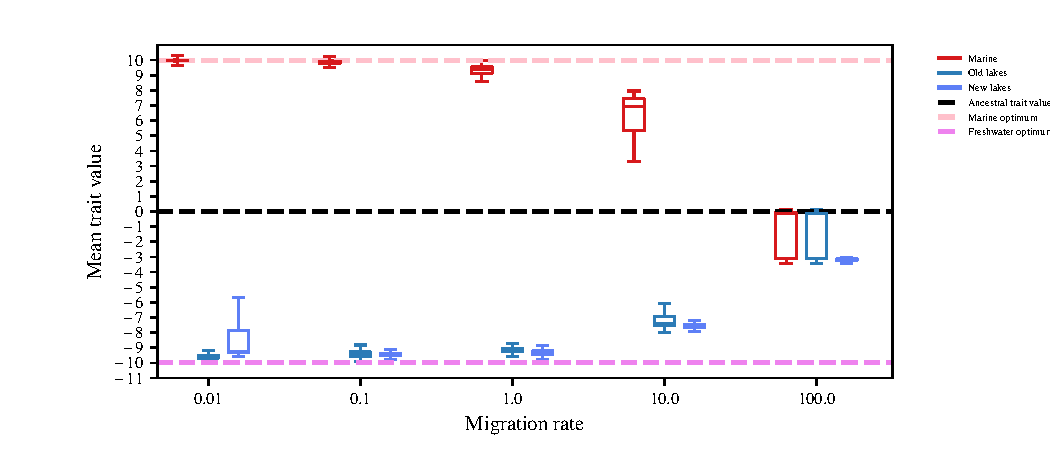
\includegraphics{Final_Plots/Pheno_Dist.pdf}
  		\caption{
            Distribution of mean trait values across generations of the simulation,
            for different migration rates.
            The dashed pink and purple lines at $\pm 10$ give the optimum phenotypes
            in the marine and freshwater environments, respectively.
		}
  		\label{fig:MeanPhenotype}
	\end{center}
\end{figure}

\begin{figure}
	\begin{center}
        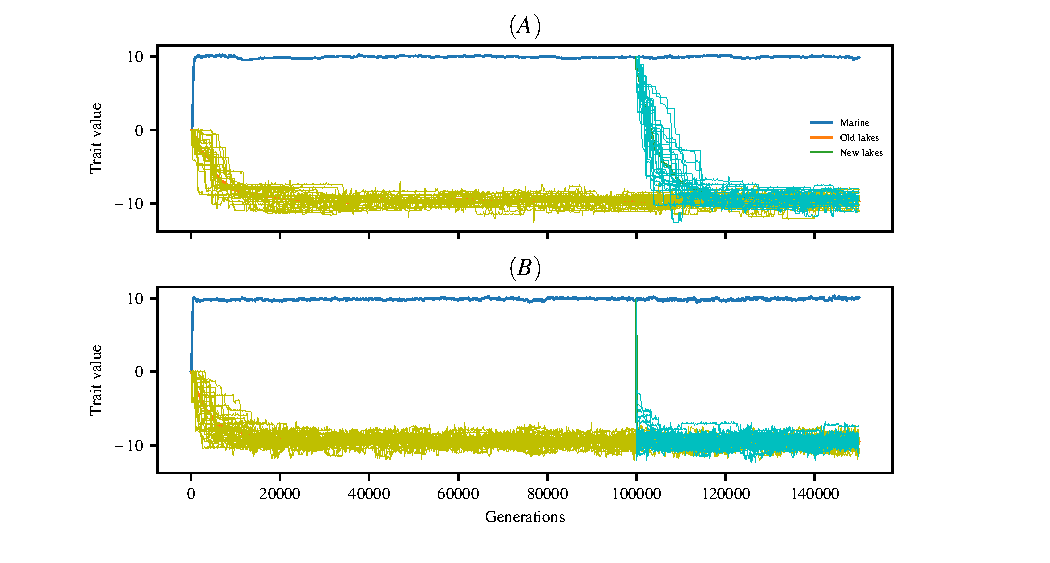
\includegraphics{Final_Plots/Pheno_Time.pdf}
  		\caption{ 
        		Mean individual trait values in the marine habitat (blue line),
        		the original lakes (yellow lines; average in orange),
        		and the new lakes (light green lines; average in dark green),
        		across the course of two simulations, with migration rates of
        		\textbf{(top)} $m=5 \times 10^{-5}$ and
        		\textbf{(bottom)} $m=5 \times 10^{-4}$ per generation per individual
        		(i.e., 0.01 and 0.1 migrants per lake per generation, respectively).
        		Optimal trait values in the two habitats are at $\pm 10$.
                	Analogous plots for other migration rates
                	are shown in Figure \ref{fig:phenotype_time_supp}.
		}
  		\label{fig:phenotype_time}
	\end{center}
\end{figure}

As shown in Figure~\ref{fig:MeanPhenotype}, local adaptation occurred at migration rates of $m \le 10$.
% with the exception of the highest gene flow at which half of each population was composed of migrants.
%At lower migration rates (10 migrants per generation and below), populations adapted to local conditions.
Figures \ref{fig:phenotype_time} and \ref{fig:phenotype_time_supp}
show freshwater and marine populations diverging until the trait means were close to the optimal values in each habitat. 
The establishment of new alleles in the lakes is visible in the first few thousand generations of Figure \ref{fig:phenotype_time} as jumps in the mean trait value.
%which move the trait by an amount of order 1 every few hundred generations.
%Trait variation within each population was small compared to the difference between populations.
At the lowest rate of gene flow, $m = 0.01$, differences at $\approx 20$ commonly polymorphic sites 
($\approx 10$ that shift the trait in each direction)
were responsible for most of the adaptive differences between freshwater and marine habitats.
In Figure \ref{fig:MPFAI}A, we can see that more gene flow simplified the genetic basis. %does this belong here?
As expected, increasing migration rate decreased differentiation between habitats. 
As seen in Figure~\ref{fig:Fst}, 
$F_{ST}$ between marine and freshwater habitats 
at neutral sites steadily declines as migration increases. 

\begin{figure}
	\begin{center}
        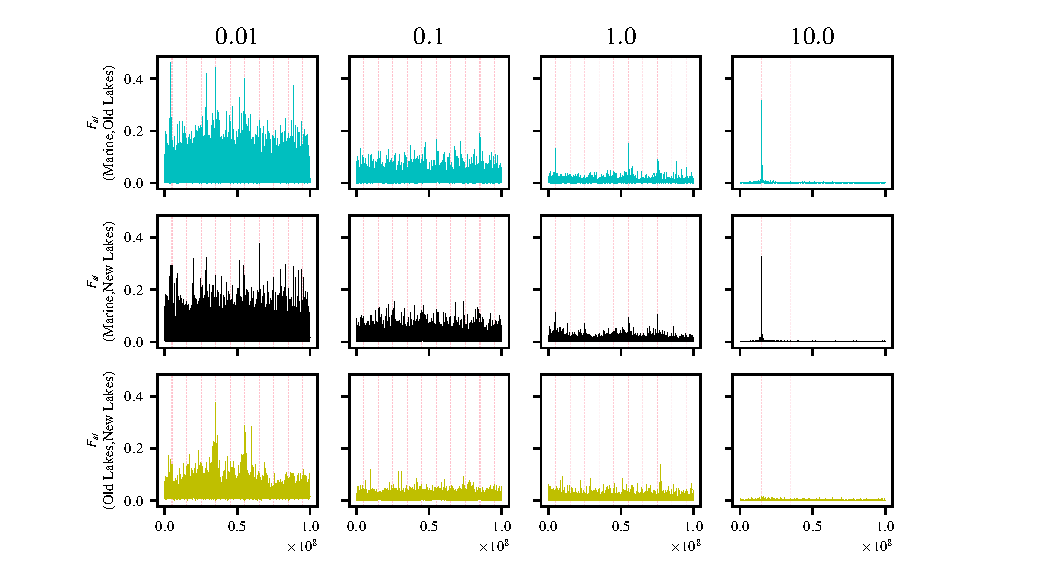
\includegraphics[width=\textwidth]{Final_Plots/Fst_Genome_faa_pos.pdf}
  		\caption{
		Average $F_{ST}$ in windows of 500Mb between:
        		\textbf{(top)} marine habitat and old lakes;
        		\textbf{(middle)} marine habitat and new lakes; and
        		\textbf{(bottom)} old and new lakes.
        		Each plot shows $F_{ST}$ values for a separate simulation,
        		with columns corresponding to increasing gene flow from left to right.
		$F_{st}$ is calculated between all marine individuals, and all lakes pooled together.
		%Ten vertical dotted pink lines in each subplot 
        		%show regions which have the potential to affect phenotype.
		All locations of pre-existing freshwater adapted alleles have been highlighted by 
		pink dashed vertical lines with an alpha value of 0.3, so darker shades of blue imply more 
		freshwater adapted alleles at that location.
     } \label{fig:Fst}
	\end{center}
\end{figure}

\paragraph*{Speed of adaptation}
Adaptation occurred much more quickly
at higher migration rates,
both in the old and new sets of lakes.
We measured this ``time to adaptation''
as the number of generations until 
average trait values in old and new lakes were within 0.5 of each other,
shown in Figure \ref{fig:TimeToAdaptation} for different rates of gene flow.
Adaptation of new lakes took over 18,000 generations at the lowest rate of $m = 0.01$,
while at $m = 1$ migrant per, lake per generation,
new lakes managed to adapt in just under 60 generations. 
%This dramatic decrease in time to local adaptation is suggestive of just how quickly
%selection can act on standing variation. 
%It also suggests a rough threshold of gene flow required 
%to efficiently select upon the alleles present in the marine individuals. 

\begin{figure}
	\begin{center}
  		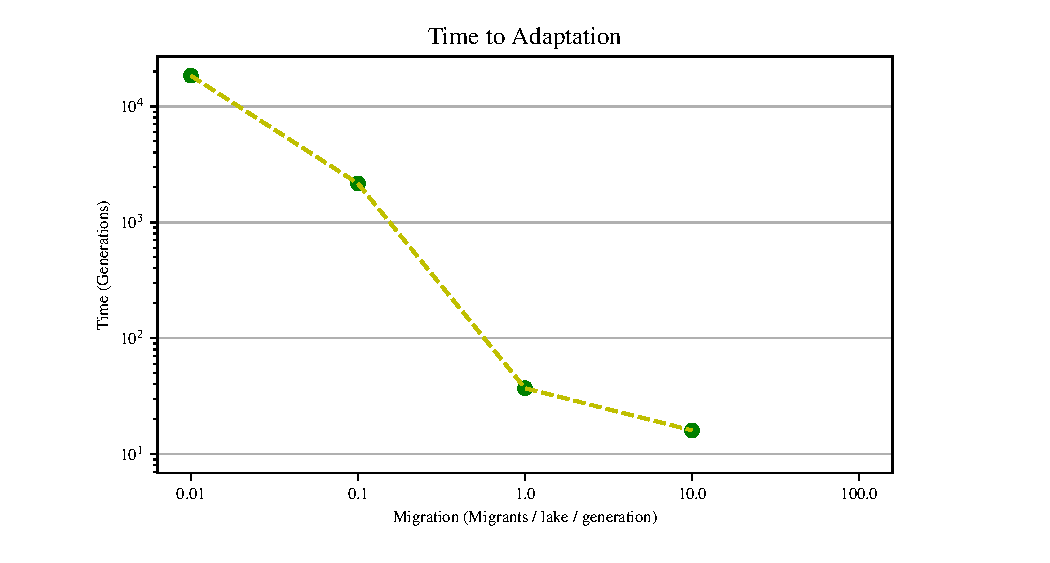
\includegraphics{Final_Plots/Time_Adapt.pdf}
  		\caption{
		Time to adaptation as a function of migration rate.
        		The time to adaptation is measured as the number of generations until
		the introduced population's mean phenotype 
        		comes within 0.5 of the original lakes average phenotype. 
		Each point represents a single simulation run.
        		(Adaptation did not occur at the highest rate of gene flow.)
        } \label{fig:TimeToAdaptation}
	\end{center}
\end{figure}

\subsection*{Sharing of freshwater adapted alleles}

At low migration rates, the \emph{initial} period of adaptation
takes roughly 25 times longer for lakes than it does for the ocean.
This difference occurs because at low migration rates,
all subpopulation must wait for novel mutations to arise in order to adapt.
Because the marine is one continuous population with 25 times more individuals than any one lake, 
there is a much larger influx of new mutations to be selected upon. 
At higher migration rates, greater mixing
allows the initial lakes to share alleles instead of developing their own genetic basis of adaptation. 
As a first indication of this, Figure \ref{fig:Fst} 
shows that $F_{ST}$ between the ``original'' and ``introduced'' sets of lakes 
at effect mutations decreased with migration rate.
%We are interested in this shared genetic basis of adaptation because it is commonly thought that this is
%a requirement for the efficient ``transportation" of the freshwater haplotype in to new lakes \citet{schluter2009genetics}

To investigate in more depth how locally adaptive alleles found in the original lakes
are shared between lakes, as well as how they spread to the new lakes,
we defined and tracked the distribution of ``pre-existing freshwater adapted alleles'' at the beginning of each generation.
To be considered in this category, a mutation must participate in the genetic basis of any freshwater adaptation.
Concretely, these are any non-neutral mutations whose frequency is above 50\% in at least one original lakes and below 50\% in the marine habitat.
Figure \ref{fig:MPFAI}A shows the distribution of the number of these alleles across generations.
At $m = 0.01$, each lake has a private set of about 10 mutations nearly fixed in that lake but not elsewhere:
the new lakes acquire new adaptive alleles and therefor have little to none of these adaptive alleles.
At $m = 0.1$, we again observe the original lakes adapting nearly independently from each other.
However, in Figure \ref{fig:MPFAI}A we can see the average marine individual is shown to hold $\approx 2$ pre-existing freshwater adapted alleles. 
This being the case, we can see new lakes adapt using a subset of this large repertoire of standing variation deriving from a multitude of independently derived haplotypes.
As migration rate increases past this, %we can see migration selection balance keeps the average capacity for marine individuals to carry freshwater alleles at about 2.
we can see in Figure \ref{fig:MPFAI}C that the total number of pre-existing freshwater adapted alleles declines.
%while the number of alleles which make up the genetic basis of adaptation in freshwater individuals remains relatively similar.
%Although the genetic basis seems to simplify slightly due to more , this 
This suggests that the alleles move between populations by migration 
before selection acts on new mutation for neighboring lakes.
Interestingly, the frequency of these alleles in the ocean
stays relatively constant across the reasonable rates of gene flow.

Figure~\ref{fig:MPFAI}B shows the distribution, through time, of 
the mean percentage of currently-defined freshwater adapted alleles 
that each genome in each of the populations carries.
If all individuals across lakes carried the same set of alleles determining their trait value, 
this would be 100\%. 
At the lowest migration rate $m = 0.01$,
each genome in the original lakes have almost exactly~$1/25^{th}$ 
of the total number of pre-existing freshwater adapted alleles -- 
this is because each one of the 25 lakes has adapted with a unique set of alleles. 
Since these are \emph{pre-existing} alleles, the value is zero for introduced lakes.
Figure \ref{fig:MPFAI}A shows us that at $0.1$ migrants per lake per generation and above,
the average individual across the new lakes has nearly the same amount of 
pre-existing freshwater adapted alleles as individuals across the old lakes.
As expected, the genetic basis of the freshwater phenotype 
seems to simplify as migration increases --
higher rates of migration allow
adaptive alleles of higher effect to travel more efficiently through the population,
even though they are deleterious in the ocean.

The numbers of Figure~\ref{fig:MPFAI} suggest that
the dramatic increase in speed of local adaptation we observed above occurs because
higher gene flow between populations allows sharing of freshwater alleles between populations.
%however, it is not enough for the marine population to hold bits and peices from independently formed haplotypes,
%For selection to act on SGV on the scale we observe in nature, the gene flow 
%initial generation to be able to rebuild 
We confirmed this by using recorded tree sequences to identify the origin of each trait-affecting
allele, in each individual, common in any of the new lakes at time of adaptation
as defined in the Methods.
Figure~\ref{fig:Origin} shows that at the lowest rate of gene flow the majority of adaptive alleles are derived from \emph{``de novo"} mutation.
As gene flow increases, a larger fraction of adaptive alleles 
derive from pre-existing variation in the marine population at the time of introduction.
In other words, 
greater mixing at higher migration rates allows lakes to share alleles
instead of developing their own genetic basis of adaptation.

\begin{figure}
	\begin{center}
  		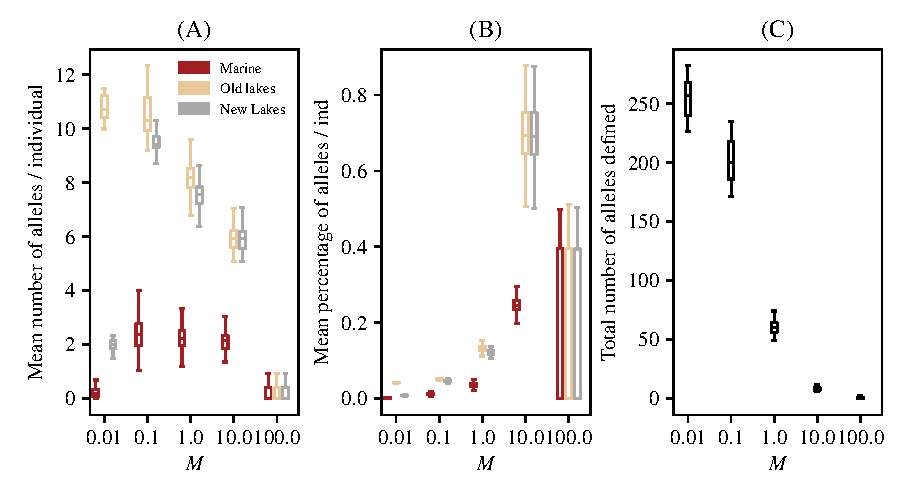
\includegraphics{Final_Plots/Freshwater_Alleles.pdf}
  		\caption{
            Amount of standing freshwater variation by habitat, across migration rates.
            Each plot counts ``pre-existing freshwater adapted alleles'',
            that are common in the original lakes but rare in the ocean
            (see text for definition).
            \textbf{(A)} Mean number of these alleles per individual.
            \textbf{(B)} Mean percentage of these alleles per individual.
            \textbf{(C)} Total number of these alleles (so, $B = A/C$).
            The number of alleles meeting these conditions changes over the course of the simulation,
            and each plot shows distributions of these values across generations.
            The horizontal axis shows $M$, the mean number of migrants per lake per generation.
		}
		\label{fig:MPFAI}
	\end{center}
\end{figure}


\begin{figure}
	\begin{center}
  		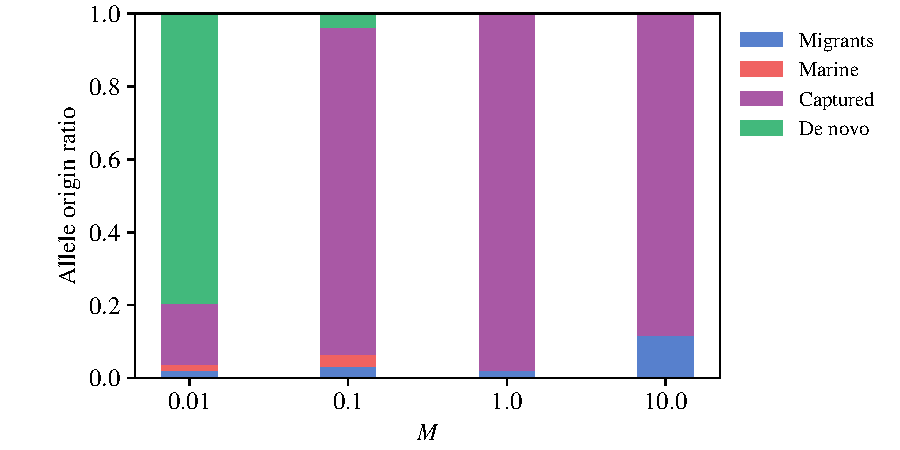
\includegraphics[width=0.7\linewidth]{Final_Plots/Allele_Origin_2.pdf}
  		\caption{ 
        		\textbf{(Origin of adaptive alleles:)}
        		Each bar plot shows the origins
		of all trait-affecting alleles above frequency 50\% in at least one new lake,
        		classified as
		\textbf{(red)} new mutations,
		\textbf{(blue)} post-colonization migrants,
		\textbf{(green)} ``captured'' from pre-existing lakes, or
		\textbf{(orange)} standing marine variation.
        		See Methods for precise definitions of these categories.
		}
  		\label{fig:Origin}
	\end{center}
\end{figure}

While increased migration allows sharing of adaptive alleles between lakes, 
at $m = 10.0$ the constant influx of alleles between the habitats creates substantial migration load. 
The rate at which migration load becomes substantial,
10 migrants per lake per generation,
only replaces 5\% of each population each generation with migrants from the other habitat, 
but this is sufficient to shift the mean trait values to nearly half their optimal values, 
as seen in Figure \ref{fig:MeanPhenotype}. 

%\begin{comment}
%\paragraph{Standing genetic variation} 
%Despite a dramatic difference in the amount of allelic sharing between lakes, 
%standing genetic variance (Figure \ref{fig:SGV}) 
%was around 0.05 in the freshwater habitat across all but the highest migration rates. 
%Concurrently, genetic variation in the marine population 
%steadily increased with migration to a similar value. 
%On the one hand, it is not surprising that lakes, as a group, 
%carry more genetic variation than the marine habitat, 
%since population subdivision allows different alleles to become common in each. 
%However, it is striking that at $m=.005$, 
%the marine habitat carries as much genetic variation, 
%despite a lack of any substantial migration load.
%\plr{perhaps we want to remove this bit? revisit if it is telling us something important.}
%\end{comment}

\subsection*{Realized genetic architecture}

Here, we take a closer look at the genomic architecture of local adaptation between the two habitats. 
Do measures of local differentiation such as $F_{st}$ scans or Genome Wide Association Studies (GWAS) identify the causal loci? 
Figure \ref{fig:Fst} shows plots along the genome of per-locus $F_{ST}$ values between the marine habitat and all freshwater habitats pooled together.
Higher rates of dispersal showed more distinct $F_{ST}$ peaks over polymorphic loci 
``Background'' levels of $F_{ST}$ increase as gene flow decreases,
swamping out this signal until the regions under selection are indistinguishable. 
This is likely the contribution of two separate forces of natural selection: 
first, stronger genetic drift with less migration leads to higher background $F_{ST}$, and 
second, greater sharing of adaptive alleles providing a shared signal across populations.

At first glance, this suggests that genome scans for local adaptation based purely on measures of differentiation 
will only be successful given enough migration between habitats. 
But how many of these peaks are actually underlying trait differences that form the basis for local adaptation?
To quantify this, Figure \ref{fig:Power_FP} shows the power and false positive rates 
that would be obtained by an $F_{ST}$ cutoff 
that declared everything above a certain value to be a causal locus.
What we observe most plainly in this graph is that $M = 1.0 \& M = 10.0$ migrants per lake, per generation
are the only rates of dispersal which provide reliable true negatives when observing peaks
This means that a large percentage of peaks past an $F_{ST}$ cutoff of $0.05$ 
actually lie on top of regions which could impact trait differences. 
Unfortunately, the low statistical power for all rates of $M$ would seem to suggest
that many regions which impact trait differences do not appear as $F_{st}$ peaks. 
This may imply that genome scans for local adaptation based purely on measures of differentiation may not be as reliable as previously thought.
To summarize, our study find that with high rates of dispersal between population, $F_{st}$ peaks may be a good indication of causal loci.
However, this is a one way implication, meaning even with high dispersal, not all causal loci will appear as $F_{st}$ peaks.


It's important to note that our study in Figures~\ref{fig:Fst} \& \ref{fig:Power_FP} pooled together all lakes and all marine individuals for the calculations. 
For comparison, Figures~\ref{fig:fst_5lakes} \& \ref{fig:Power_FP_5lakes} shows the same scans but calculated 
only on between individuals in the marine with spacial location $\le 5.0$ and the individuals in the respective 5 lakes.
These graphs show even less power and True Positives only at $ M = 10.0$ migrants per lake, per generation

%In regions of the genome underlying individual trait value, we observed 
%Given that migration increases the gene flow between subpopulations, how valid are $F_{st}$ peaks at different $M$. 
%Knowing exactly which mutations effect phenotype in our simulations, we can look at the statistical power and false positives given $F_{st}$ per SNP across the genome.
%In Figure \ref{fig:Power_FP} , looking at an $F_{st}$ threshold greater than 1, we see the two lowest migration rates $10^{-5}$ and $10^{-4}$ having very little statical power. 
%This along with low false positive rate across all $F_{st}$ threshold values is fairly predictable when you consider the high $F_{st}$ values across the genome. 


\subsection*{Origin of introduced freshwater adaptive alleles}

We have thus far found that the speed of adaptation depends strongly
on the degree to which alleles can be shared between populations.
However, the large increase in speed of adaptation between dispersal rates of $M = 0.1 \& M = 1.0$, seen in Figure \ref{fig:TimeToAdaptation}, remains a mystery. 
Figure~\ref{fig:MPFAI}A shows that with $M = 0.1$ migrants per lake per generation, 
there is substantial sharing of alleles between populations,
and yet at this rate new lakes take around 2,000 generations to adapt.
This is surprising because we see a similar quantity of allele sharing at  $m = 1.0$, 
but much more rapid adaptation ($\approx 60$ generations). 
A reasonable explanation for this 33$\times$ discrepancy is that 
new lakes must wait for an additional influx of freshwater alleles through migration
beyond what is present in the initial generation.
This hypothesis is disproven by
Figure~\ref{fig:Origin}, which shows that at both $m = 0.1$ and $m = 1.0$,
the vast majority of alleles underlying the local adaptation
derived from individuals in the original generation (``captured'').

\begin{table}[ht]
    \centering
    \begin{tabular}{rrrrr}
      \hline
     & m=0.01 & m=0.1 & m=1 & m=10 \\ 
      \hline
          best & 2.77 & -12.02 & -21.02 & -7.02 \\ 
      % expected & 4.22 & -4.78 & -14.64 & -5.47 \\ 
       \hline
    \end{tabular}
    \caption{
        Haplotypic variation present in the new lakes at time of colonization,
        across rates of gene flow,
        % \textbf{``Best''} 
        quantified as the most negative trait value achievable
            with intact haplotypes, averaged across populations
            (see text for details).
        % \textbf{``Expected''} shows the trait value
        %     achieved by averaging haplotypic values weighted by fitness
        %     (see text for details).
    } \label{tab:linkage}
\end{table}

An alternative explanation is that at lower rates of gene flow,
freshwater alleles present as standing variation in the marine habitat
are more tightly linked to marine alleles.
This implies the adaptation in the new lakes must wait for recombination to break freshwater adapted alleles from nearby marine adapted alleles.
This might be expected at low dispersal rates since freshwater alleles present in the ocean
%to remain present at migration-selection balance at low migration rates,
must be ``masked'' by nearby compensatory alleles.
Without masking their affect on phenotype, they would likely be pushed out by drift.
Reversing this ``masking'' then slows the process of adaptation that uses this genetic variation.
In other words, higher dispersal from freshwater to the ocean maintains relatively intact freshwater haplotypes
that can be more easily rebuilt in the marine environments.
Recall from our description in methods, that trait-affecting mutations only occur in relatively small regions of $10^5$ loci
in which recombination occurs in these regions only once in every one thousand meioses.
This implies that even if there is a sufficient amount of variation in the initial population of a lake
to shift the trait from the marine optimum ($+10$) to the freshwater optimum ($-10$),
rebuilding the most beneficial haplotype may prove to be a non-trivial task for selection.
%these may be tightly linked to alleles that counteract their effect.
For example, suppose there are 10 variants segregating at low frequency with effect size $-1$ each,
but each is paired with a compensatory allele with effect size $+1$.
Each local haplotype is therefore neutral.
This would also explain why at low rates of dispersal 
the marine still has the capacity to hold a large amount maladaptive alleles within the individuals of its population, 
as seen in \ref{fig:MPFAI}A.
%(and so likely to be at higher frequency in the marine population).

%Indeed, this appears to be the case.
To quantify the genetic variation available \emph{without} recombining within the ten genomic regions,
we first found, within each population, the haplotype with the largest net negative effect
at each of the ten genomic regions.
Summing these ten numbers, 
we get the maximum amount that selection could move the population in the freshwater direction
without recombining \emph{within} selectively non-neutral regions.
The mean of this value across the 25 lake populations is shown 
in the (``best'') row of Table~\ref{tab:linkage} --
typical populations at $M=0.1$ migrants per lake per generation could shift to a phenotype of -12.02
(and so have sufficient variation to adapt without recombination),
but the ``best'' haplotypes in the populations at $M=1.0$ have effect sizes nearly twice as big at a mean total of -21.02.
Confusingly, at $M=10.0$ the best haplotype then raises to an unimpressive -7.02.
However, this can simply be explained by the migration load the populations are experiencing, explained earlier and seen in Figure~\ref{fig:MeanPhenotype}

\subsection*{Theoretical expectations}

We now revisit our observations above
in the light of population genetics theory.
The discussion will be rough,
with a focus on intuition rather than precise calculations.
Since within each population we model stabilizing selection on an additive trait
controlled by a moderately large number of loci,
more precise expectations might be obtained through quantitative genetics \citep{svardal2014general}
or even Fisher's geometric model \citep{barton2001hybridization,chevin2014niche}.

Suppose a new allele enters a lake, either by migration or mutation. 
If, when it is rare but present in $n$ copies, it has fitness advantage $s$ 
-- i.e., the expected number of copies in the next generation is $(1+s)n$ 
-- then the probability that it escapes demographic stochasticity to become common in the population 
is approximately $2s$ \citep{lambert2006probability,haldane1927mathematical}
(assuming Poisson reproduction, as we roughly have here).
If the current population all differed from the optimum trait by $z$, 
and the allele has effect size $-u$ in heterozygotes, 
then the fitness advantage of the allele would be $s(u) = \exp(-\beta((z - u)^2) / \exp( - \beta z^2)) \approx 2 \beta z u$, where in our parameterization, $\beta = 1 / 450$. 
This tells us two things: (1) the rate of adaptation decreases as the population approaches the optimum, and (2) larger mutations (in the right direction) are more likely to fix.

\paragraph{New mutations}
The total rate of appearance of new mutations per lake is $\mu_L = 0.04$, 
which are divided evenly in seven categories: neutral, and then additive, dominant, and recessive in either direction. 
This implies that a new additive or dominant effect mutation appears once every 87.5 generations, on average. 
Effect sizes are randomly drawn from an Exponential distribution with mean $1/2$, 
and so the probability that a dominant mutation manages to establish in a population differing from the optimum by $z$ 
is roughly $\int_0^\infty 4 \beta z u \exp(-2u) du = \beta z$, 
and so the rate of establishment of dominant mutations is $\beta z / 87.5$, 
i.e., about one such mutation every $2461/z$ generations. 
The distribution of these successfully established mutations 
has density proportional to $u \exp(-2u)$, i.e., is Gamma with mean 1 and shape parameter 2. 
Since additive alleles have half the effect in heterozygotes, 
they have half the probability of establishment. 
During the initial phase of adaptation, the populations begin at around distance $z=10$ from the optimum. 
Combining these facts, we expect adaptive alleles to appear through mutation within lakes at first on a time scale of 250 generations, 
with the time between local fixation of new alleles increasing as adaptation progresses, and each to move the trait by a distance of order 1.
This agrees roughly with what we see in Figures~\ref{fig:phenotype_ts2} and XXX.
\plr{refer to additional trace plots in the supp}

\paragraph{Standing variation}
An allele that moves the trait $z$ units in the freshwater direction in heterozygotes 
has fitness roughly $\exp(-\beta z^2) \approx 1 - \beta z^2$ in the marine environment. 
The product of population size and fitness differential in the marine environment for a mutation with $z=1$ is therefore $2Ns = 8.9$, 
implying that these alleles are strongly selected against but might occasionally drift to moderate frequency. 
The average frequency of such an allele in the marine environment at migration-selection equilibrium 
is equal to the total influx of alleles into the ocean per generation divided by the selective disadvantage, 
which if there are $M$ immigrants per generation, is $2 M / \beta z^2$. 
\plr{This $M$ is the total number in the ocean! Make sure this differs from notation above for the number per lake.}
Each new lake is likely to contain a few copies of alleles at frequency above 1/400
(since each new lake is begun with 400 genomes).
With $z=1$, the factor multiplying $M$ is $2/\beta z^2 \approx 1/200$,
so if $M \ge 1$, 
the chances are good that any particular lake-adapted allele that is present in all pre-existing lakes 
will appear at least once in the fish that colonize a new lake. 
However, an allele with $z=1$ only has probability of around 1/20 of establishing locally, 
suggesting that the migration rate should be somewhat higher to ensure enough pre-existing genetic variation 
that adaptation would happen entirely using the initial set of colonizers. 
% This corresponds to our highest two migration rates, as in e.g., Figure \ref{fig:phenotype_ts2}B.
However, this calculation treats each allele independently;
in practice we found that standing freshwater variation in the ocean
were masked by linkage to compensatory marine variants.

\paragraph{Migration}
The key quantity regulating the amount of standing variation in the ocean was the \emph{downstream} migration rate,
from lakes to the ocean.
How important is the upstream migration rate?
If sufficient genetic variation is not present in a new lake initially, 
it must appear either by new mutation or by migration. 
Since a proportion $m$ of each lake is composed of migrants each generation, 
it takes $1/m$ generations until the genetic variation introduced by migrants equals the amount initially present at colonization. 
This implies a dichotomy: either 
(a) migration is high, and adaptation is possible using variants present at colonization or arriving shortly thereafter, or 
(b) migration is low, so adaptation takes many multiples of $1/m$ generations.
Since in our model lower migration also reduces the amount of variation available in the ocean,
we expect very little contribution of subsequent migration across any value of $m$,
as seen in Figure~\ref{fig:Origin}.

% These calculations depend on there being no bottleneck in colonization of the lake; if there is a bottleneck, then an additional factor must be added. At what point do we expect new mutation to be more important than migration for adaptation? By the calculations above, if $M \ge 10$, we expect initial diversity in a lake to be sufficient  for adaptation, corresponding to our third-highest migration rate. If this does not happen, then we expect adaptation to take a multiple of $1/m$ generations;
% with our values, $1/m$ ranges from 20,000 to 20 generations. Above we estimated that adaptive alleles due to new mutation fix locally about every 2,000 generations, suggesting that at our second-lowest migration rate (where $1/m = 2,000$), the two contributions of migration and new mutation are roughly equal.
% This is in fact what we see: in Figure \ref{fig:MPFAI}, we see that at the second migration rate, alleles start to be shared between lakes, while by the third migration rate, they are almost entirely shared.

%%%%%%%%%%%%%%%%%%%%
\section*{Discussion}
 
In this paper, we have described a realistic simulation model of a coastal metapopulation to observe the effects of selection of genetic variation (SGV) across a wide range of gene flow rates.
We have shown that historical introgression, at our given parameter sets, is able to reproduce rapid and parallel adaptation similar to what we've seen in real populations such as Middleton island. 
Selection is able to rebuild the freshwater haplotype at a rapid pace (in tens of generations) from marine populations as a medium between all freshwater populations. 
Almost all rates of migration were helpful in the efficiency of the population to locally adapt except for the highest at which migration load limited the ability of the populations to reach the local optimum. 

While our findings prove useful to the understanding of stickleback, they are not autonomous to this species. 
Now, we will discuss the broader implications of our findings on the more general framework of similar systems, we also explore what other questions remain. 
Small patches of similar selective pressures can be found in many places such as high altitudes, underwater volcanic vents, or post forest fire environments. 
%We are still finding new subspecies, that seem to have adapted to extreme environments presented in small patches connected to larger spanning biospheres where the ancestral species naturally inhabits.
Recently, (Cite Nelson Ferretti et al), discovered seven new species of Hapalotremus (Theraphosinae), living at the extremely high altitudes distributed along the Andes and Yungas in western South America.
With the ancestral species at much lower altitudes, beneficial high altitude alleles could potentially be carried to help in the colonization of neighboring mountain environments. 
Systems of metapopulations like this could potentially arise in many places
where the ancestral species carries around with it beneficial alleles forselective pressures it has encountered in the past and remains connected to through hybridization events.
 
%(1) the subspeciesthat inhabits a different selective pressure, and ancestral species are not constrained by pre, or post-zygotic isolation to participate in hybridization events, and
%(2) the ancestral species spans across a wide range. 
%For brevity, I will call evolutionary systems which satisfy these conditions, 
%The vast number of species which encou
 
 \paragraph{Atmosphere's ability to carry whoever scotty is beaming up ... }
Perhaps the most notable finding in this study is that large, ancestral populations have the capacity to maintain alleles which are potentially deleterious for an extended amount of time.  
%This system seems analagous the marvel superhero \emph{Rogue}, who can steal superpowers or memories from another  for a limited amount of time as long as she has contact with the indivi
This principle, deriving solely from the properties of sex and natural selection, could be applicable to almost any species experiencing the influence of divergent selection with introgression.
And to explore further how this process is carried out exactly, many of the questions lie in understanding which properties of genomic architecture and demographics allow this transportation to be possible. 
%In terms of Star Trek's ``transporter" referred to by \citet{schluter2009genetics}, 
his is largely analogous to exploring the specific properties of the atmosphere / space which allow for the heroes to be disassembled, then put back together.
%While the perspective of our 
In our simulations, the continued gene flow from freshwater populations meant that the alleles were maintained at a constant rate with fixed demographics. 
Two possible questions that might arise from this are:
(1) How do population sizes, demographics, and evolutionary histories impact an ancestral population's capacity for carrying maladaptive alleles in its opposing environment, and 
(2) What role does genomic architecture play in the ability for a haplotype to be rebuilt.
 
\paragraph{Origins of genetic basis of local adaptation in new lakes}
In Figure~\ref{fig:Origin} we found that the genetic basis for local adaptation, when selecting upon SGV, is propogated largely from the initial generation of inhabitants. 
This contrasts the belief that subsequent migration is a necessity in newly established populations ability to rebuild a haplotype.
This finding suggests that with high probability, a randomly chosen subset from ancestral species in the metapopulations like marine stickleback, 
carry the capacity to rapidly adapt without \emph{any} continued connection to the rest of of the species.

\paragraph{Realized genomic architecture}
Additionally have also shown introgression is beneficial for inferring causative loci from divergence ($F_{st}$) along the genome. 
This is generally because noise of selectively neutral alleles divergence can appear causative when genetic drift causes more 
differences between populations that have little gene flow between them.
It's important to know that in all scenarios, hitchhiking of selectively neutral alleles could also be 
mistaken for being causative as they often display the same amount of divergence.

%\paragraph{Implications for the ``Transporter"--hypothesis}





%%%%%%%%%%%%%%%%%%%%%%%%%%%
%DO WE NEED THIS?
\begin{comment}
\subsection*{thresholds}

We have found that too little migration leads to selection upon new mutations in all subpopulations and lakes alike. In contrast, at high migration rates we have seen that migration load limits the ability for species to locally adapt to the selective pressure of their environment. This leads us to consider a window of introgression which allows for the transportation of FAA's without migration load. 

\subsection*{connect results back to real data?}

\paragraph{The adaptive filter?}
RAMBLING THOUGHTS HERE
Since larger effect alleles are more likely to establish,
be it by mutation or migration,
repeated colonization of new freshwater habitats will select for larger alleles,
be it single alleles or haplotypes bound together by an inversion.
However, these are more strongly selected against in the interstitial time.
Being recessive would help with this,
but would also make it more difficult to establish.

\jgg{TODO: effect of smaller than realistic population sizes?}

\jgg{TODO: Talk about the role recombination plays}
This also brings to light the role of recombination in a system of migration selection balance. 
On one hand, a lower recombination rate would allow for the freshwater haplotype to remain "intact" 
within the marine environment, however, without significant introgression the haplotype would quickly get selected against in marine populations. 
On the other hand a higher recombination rate would, in theory, allow freshwater adapted alleles more longevity 
as they would hitchhike with marine adapted haplotypes. 


\paragraph{Modeling assumptions}
Our simulations had much smaller population sizes than real populations.
How might this affect things?
\end{comment}
%%%%%%%%%%%%%%%%%%%%%%%%%%%%

\bibliographystyle{plainnat}
\bibliography{Citations}{}

%%%%%%%%%%%%%%%%%%%%%%%%%
\clearpage
\appendix
\setcounter{table}{0}
\renewcommand{\thetable}{S\arabic{table}}
\setcounter{figure}{0}
\renewcommand{\thefigure}{S\arabic{figure}}


\section*{Supplementary material}

\begin{figure}
	\begin{center}
  		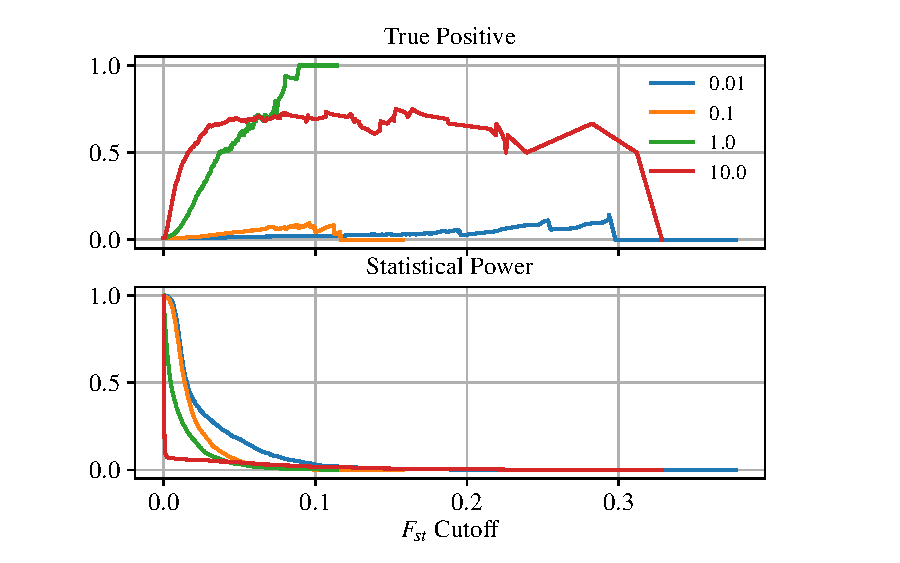
\includegraphics{Final_Plots/True_Power_0_25_500.pdf}
  		\caption{ 
		Statistical Power and False Positives as a function of $F_{st}$ threshold. 
		Statistical Power is the likelihood that a SNP will be predicted to have an effect on phenotype when there is an effect to be detected (?).
		False Positives give us the ratio of SNPs that effect phenotype to total SNPs greater than the $F_{st}$ threshold.
            \textbf{
                TODO: fix this caption; x-axis label ($F_{ST}$).}
		}
  		\label{fig:Power_FP}
	\end{center}
\end{figure}

\begin{figure}
	\begin{center}
		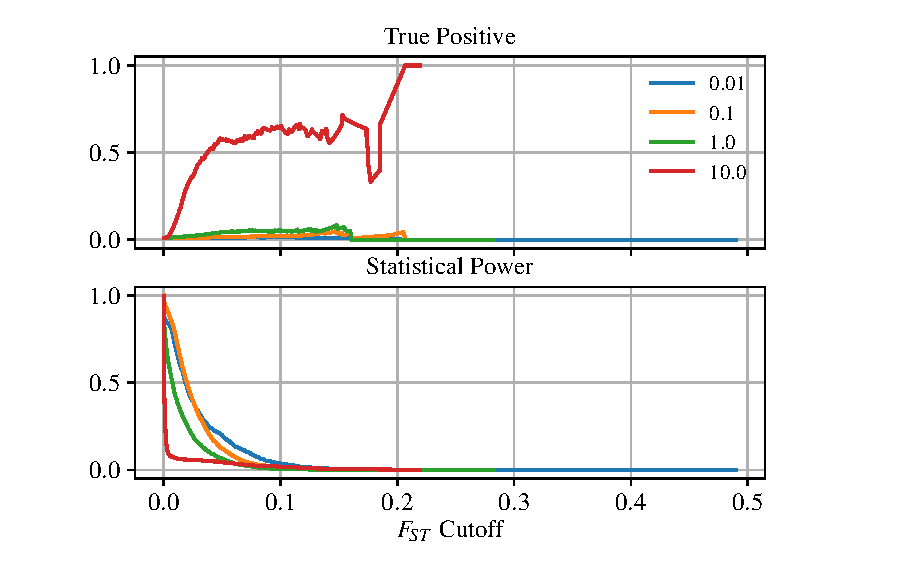
\includegraphics{Final_Plots/True_Power_0_5_500.pdf}
  		\caption{ 
		Statistical Power and False Positives as a function of $F_{st}$ threshold. 
		Statistical Power is the likelihood that a SNP will be predicted to have an effect on phenotype when there is an effect to be detected (?).
		False Positives give us the ratio of SNPs that effect phenotype to total SNPs greater than the $F_{st}$ threshold.
            \textbf{
                TODO: fix this caption; x-axis label ($F_{ST}$).}
		}
  		\label{fig:Power_FP_5lakes}
	\end{center}
\end{figure}

\begin{figure}
	\begin{center}
  		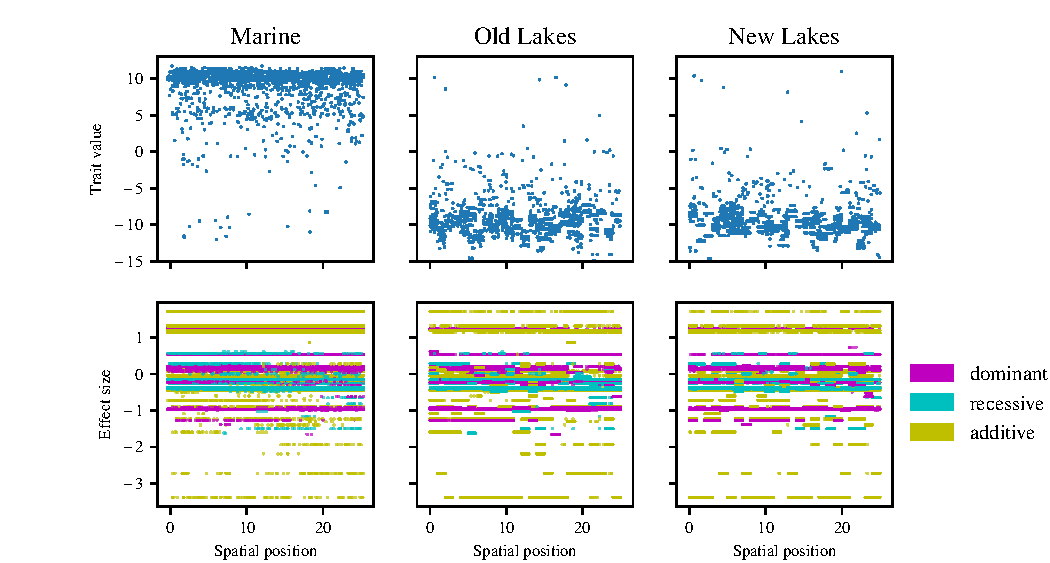
\includegraphics[width=1.0\linewidth]{Final_Plots/Haplo_small.pdf}
  		\caption{
			Phenotypes (\textbf{Top}) (effect size and mutation type) and haplotypes \textbf{(Botton)} as a function of spatial position of the individual 
			possessing the genome. The phenotype of each haplotype is, by definition, the sum of the 
			effect sizes of each mutation in the genome. 
		}
  		\label{fig:Haplo_Pheno}
	\end{center}
\end{figure}


\begin{figure}
	\begin{center}
  		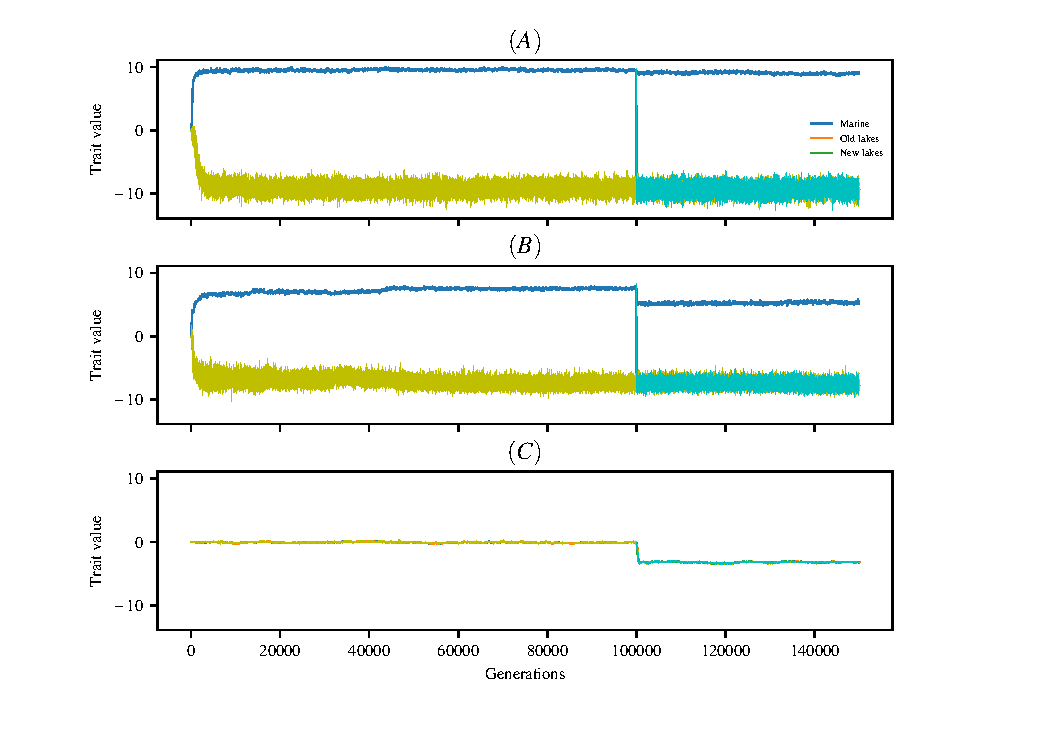
\includegraphics[width=1.0\linewidth]{Final_Plots/Pheno_Time_supp.pdf}
  		\caption{
		Mean individual trait values in the marine habitat (blue line),
        		the original lakes (yellow lines; average in orange),
        		and the new lakes (light green lines; average in dark green),
        		across the course of two simulations, with migration rates of
        		\textbf{(A)} $m=5 \times 10^{-3}$,
        		\textbf{(B)} $m=5 \times 10^{-2}$ and
		\textbf{(B)} $m=5 \times 10^{-1}$.
        		(i.e., 1, 10, and 100 migrants per lake per generation, respectively).
        		Optimal trait values in the two habitats are at $\pm 10$.
		}
  		\label{fig:phenotype_time_supp}
	\end{center}
\end{figure}

\begin{figure}
	\begin{center}
  		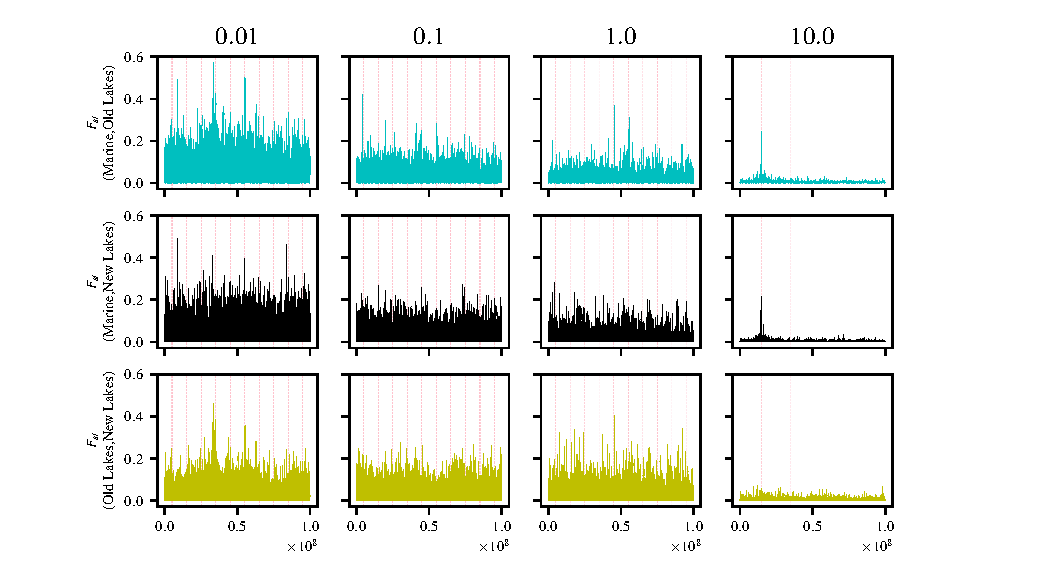
\includegraphics[width=1.0\linewidth]{Final_Plots/Fst_Genome_faa_0_5_500.pdf}
  		\caption{
		Average $F_{ST}$ in windows of 500Mb between:
        		\textbf{(top)} marine habitat and old lakes;
        		\textbf{(middle)} marine habitat and new lakes; and
        		\textbf{(bottom)} old and new lakes.
        		Each plot shows $F_{ST}$ values for a separate simulation,
        		with columns corresponding to increasing gene flow from left to right.
		$F_{st}$ is calculated between all marine individuals with spatial location $\le 5.0$, and the five corresponding lakes.
		All locations of pre-existing freshwater adapted alleles have been highlighted by 
		pink dashed vertical lines with an alpha value of 0.3, so darker shades of blue imply more 
		freshwater adapted alleles at that location.
		}
  		\label{fig:fst_5lakes}
	\end{center}
\end{figure}

\end{document}



The calculation above ignores allele frequencies -- 
even if a population \emph{could} adapt entirely using the best possible haplotypes,
many of these may be lost to drift.
To account for this, we calculated a similar quantity but accounting for the probability of fixation.
Suppose that the alleles present in the initial population of a new lake
have effect sizes $(x_1, \ldots, x_n)$,
and that the probability of fixation of a single allele of effect size $x$ is $p(x)$.
Let $X_i$ be the average per capita effect of the $i^\text{th}$ allele after fixation,
so that $X_i = 0$ if the allele is lost,
and $X_i = 2x_i$ if the allele fixes (ignoring dominance).
Therefore, the expected contribution to the final trait value of allele $i$
is $\E[X_i] = 2 x_i p(x_i)$.
The trait value after the initial round of adaptation is $\sum_i X_i$,
and so the expected trait value is $2 \sum_i x_i p(x_i)$.
Since there are many alleles that contribute more-or-less additively to the trait,
the probability of fixation of a particular allele is not easy to find,
but we can roughly approximate it as follows:
if the current population trait mean $z$,
then an allele that moves the trait a distance $x$ closer to the optimum
has a fitness advantage in heterozygotes of 
$\exp(-\beta((z - x)^2) / \exp( - \beta z^2)) \approx 1 + 2 \beta z x$, 
where in our parameterization, $\beta = 1 / 450$.
Since the probability of fixation of a single allele with relative advantage $s$
is approximately $2s$ \citep{lambert2006probability,haldane1927mathematical},
then with $z=10$ we can use $p(x) \approx 4 x / 45$.
Putting these considerations together,
a rough estimate for the total shift in trait value resulting from selection
on standing variation in the initial population is
$R = \sum_i 8 x_i / 45$,
where the sum is over all trait-affecting alleles.
This approximation should be good if each trait-affecting allele is rare (present in only a few copies),
effects are additive, and most are unlinked.

We computed $R$ to confirm our suspicion that linkage slowed down adaptation
by showing that there is sufficient allelic variation in the initial populations
to complete adaptation across both migration rates (0.1 and 1 migrants per lake per generations),
but not if the haplotypes of each genomic region are assumed to not recombine.

We calculated for each individual in the initial generation of the new lakes
the total contribution to trait values of each of the ten genomic regions 
that containing trait-affecting mutations.
The recombination rate within each of these ten regions is $10^{-2}$,
so these regions act initially more-or-less like single loci.
Even though the trait is additive across loci,
the presence of sufficiently many distinct alleles to attain, in principle,
the optimal freshwater trait value
does not ensure adaptation will actually occur with these alleles.
On the contrary, many of these will likely be lost to drift.

Between $m = 0.1$ and $m = 1.0$ we see a large difference in the total effect sizes of the haplotypes that are expected to fix.
Given these numbers were computed assuming additivity (slight overestimate) and individuals are diploid,
at $m = 0.1$ the mean total genotype expected to fix in the populations puts individuals at a trait value of $\approx -8$ 
after selection on alleles haplotypes in the initial population. 
In turn, the population must wait for novel mutation or subsequent migration to provide the alleles for the remaining 2 units before 
attaining a mean average trait value at the optimum (-10).
It follows in Figure \ref{fig:phenotype_ts2}B that the majority time to adaptation is spent within 2 units of mean trait value.
The initial adaptation on selection of standing variation up to that point happens quite rapidly.
This provides evidence that linkage to marine alleles has a major impact in the introduced population's ability 
to select and rebuild a pre-existing haplotype given the standing variation at time of introduction. 

